% sage_latex_guidelines.tex V1.20, 14 January 2017

\documentclass[doublespace,times,Afour,review]{template/sagej}

\usepackage{moreverb,url}

\usepackage[colorlinks,bookmarksopen,bookmarksnumbered,citecolor=red,urlcolor=red]{hyperref}

\begin{document}

\runninghead{Ritwiz Sarma and Riju Garg}

\title{The Himalayan Tightrope: A High-resolution Study of the Economy-Environmental Trade-off of Infrastructure Development}

\author{Ritwiz Sarma\affilnum{1} and Riju Garg\affilnum{2}}

\affiliation{\affilnum{1}Madras School of Economics.\\
\affilnum{2}Madras School of Economics.}

\corrauth{Ritwiz Sarma, Graduate Student, Madras School of Economics, 1 Ranjith Road, Kotturpuram, Chennai, Tamil Nadu IN.}

\email{ge23ritwiz@mse.ac.in}

\begin{abstract}
This paper uses modern high-resolution data on growth and environmental degradation to analyze the trade-offs between economic development and ecological conservation amidst infrastructure development in the northern Himalayan region. We use novel satellite-based data sources to capture highly localized effects of development and attempt to investigate the levels of efficiency currently possible in building infrastructure in sensitive biomes. Development processes, however, remain inseparable from environmental degradation, even with new advances in clean energy. It thus becomes relevant to explore levels of efficiency, ie. the environmental cost to economic development, that is currently possible in infrastructural development. We use a novel geospatial and temporal dataset which combines economic and environmental indicators to investigate localized effects of development processes to compare efficiencies amidst different situational and policy contexts. The study also adds to the growing literature on the development vs. conservation trade-off by capturing a unique view of the opposing forces at play in a biome of great significance to India and the rest of the world.

\end{abstract}

\keywords{Economy-ecology tradeoff, infrastructure development, satellite data, geospatial data}

\maketitle



\section{Introduction}
The “great purpose” of development economics is to build a world where the country of your birth does not “dictate your potential as a human being.\endnote[1]{Quote often attributed to Gen. Romeo Dallaire, the famed UN peacekeeper and Canadian senator.}”  Over the past few decades, the growth of environmental awareness has often conflicted with development, courtesy of the intuition that there exists a zero-sum game between environmental protection and economic development. This paper delves into this perceived tradeoff using new-age satellite-based data sources to focus on a specific biome of exceeding importance, the Himalayas.

The Himalayan mountain range has always been considered a boon to India in terms of the natural resources, economic support, and natural defence that it provides. Development in the Himalayas, however, has been contentious: on one hand, there has been rapid infrastructural development and investment by the government, in order to increase the connectivity of the Himalayan states with the rest of the country and extract more economic benefits through avenues such as tourism. On the other hand, nudges to the fragile environmental ecosystem of the Himalayas has been connected to their increased vulnerability to disasters - the most notable example being the 2023 land subsidence incident at Joshimath, Uttarakhand (Sharma, 2023).

There exists a substantial literature on the economy-environment trade-off, especially building on the Environmental Kuznets Curve, which predicts an inverse-U-shaped relationship between economic growth and environmental degradation (Dasgupta et al., 2002; Ekins, 1997; Nguyen \& Malesky, 2021; Porter \& van der Linde, 1995). These estimations are often made from large-scale macroeconomic data at the level of countries. This study uses high-resolution temporal data, which allows us to narrow our focus to the Himalayan states of Himachal Pradesh and Uttarakhand, while also preserving statistical richness in the data to make inferences possible. 

The following section provides further context on the economy-environment tradeoff and its intersection with the Indian policy backdrop. The third section describes our data across our temporal range and introduces our panel model to study the impacts of change in the environmental indicators on the nighttime lights data, which is being used as a signal of infrastructure development. The fourth section summarizes our results, and the final section concludes.



\section{Context}

\subsection{Competing Motivations}

The infrastructural development of the Himalayan region is vital for India from three perspectives: economic, political and administrative. 

The economic perspective highlights the importance of investment in the Himalayan region with the help of infrastructural development like roads and dams in order to spur network effects and increase efficiency. Roads are essential amidst the mountainous terrain to improve connectivity provide livelihoods through tourism. Uttarakhand is shifting from being an agriculture-based economy to one focusing on manufacturing and services. The primary sector provided for 10.2\% of GSDP in 2019-20 – a steep fall from a lofty 31.49\% in 1999-2000. The provision of livelihoods in Himachal Pradesh has increasingly become a political concern, especially since no political party has dominated state elections. Road-building in particular remains a politically-favoured form of public investment, mainly because of its visible nature which promises electoral returns. From the administrative perspective, building infrastructure deepens and strengthens the reach of the state. 

The strategic location of the Himalayas is another reason to promote infrastructural development. It connects India with the neighboring countries China, Nepal and Bhutan. The India-China Border Roads (ICBR) in response to Chinese infrastructure development along the border. The project includes construction of strategic roads, including bridges and tunnels. The improved connectivity is also vital for commuting of artillery and infantry, thereby ensuring increased security.

However, the Himalayan states have a record of natural calamities propelled by development processes: the 2013 Uttarakhand floods prompted discussion on overexploitation of natural resources and the awareness for sustainable development. Ten years later, the Himalayan region was struck by the Joshimath land subsidence incident in 2023. Though the government has tried to initiate programmes like Himalaya Diwas to protect the ecosystem, the results have not been satisfactory.

\subsection{Theoretical Framework}

The Environmental Kuznets Curve (EKC) was introduced with the hypothesis that there exists an inverted U-shaped relationship between environmental degradation and national income\endnote[2]{The original Kuznets curve, introduced by the Russian economist Simon Kuznets, dealt with inequality and economic growth.}. It was developed by Grossman and Krueger (1991) who analyzed the linkage between economic growth and environmental pollution. They used four types of indicators: urban air pollution, the state of the oxygen regime in river basins, fecal contamination of river basins, and contamination of river basins by heavy metals. They postulated that the initial stages of economic growth are noted to be associated with increased environmental degradation due to increased exploitation of natural resources, production, and industrialization. They divide the economic growth into three periods: pre- industrial economy, industrial economy and post- industrial economy. Therefore, environmental degradation may be inevitable in developing regions where countries have either embarked on or are in the process of embarking on the path to development.


\begin{figure}[h]
    \centering
    \includegraphics[width=0.4\textwidth]{images/kuznets_scen.png}
    \caption{Different scenarios for the Environmental Kuznets curve (Dasgupta et al., 2002).}
\end{figure}


There have been studies contradicting the EKC as well. Stern (2004) points out that the EKC is econometrically weak and that the empirical support for the EKC is mixed. S. Dasgupta et al. (2002) presented evidence that contradicted the typical EKC pattern. Similarly, the shape of the Kuznets curve has been disputed over the past decades (Caviglia-Harris et al., 2009, Dimitra \& Efthimios, 2013, List \& Gallet, 1999). 



\section{Data}

\begin{table}[b]
    \centering
    \begin{tabular}{|l|r|r|r|r|}
    \hline
    \multicolumn{1}{|c|}{\textbf{Variable}} & \multicolumn{1}{c|}{\textbf{Mean}} & \multicolumn{1}{c|}{\textbf{Std. Dev.}} & \textbf{Min} & \textbf{Max} \\ \hline
    Built-up area                           & 69.70                             & 107.06                                  & 0.00            & 1570.46      \\ \hline
    Night-lights                            & 2.19                              & 4.21                                   & 0.00            & 63.00           \\ \hline
    Forest cover                            & 24.89                              & 8.42                                    & 79.62        & 120.00          \\ \hline
    PM2.5                                   & 31.50                              & 7.83                                    & 12.79        & 77.00           \\ \hline
    LST                                     & 25.51                             & 9.23                                   & 21.42       & 36.20       \\ \hline
    \end{tabular}
    \caption{Descriptive statistics. \label{table:descstats}}
\end{table}


Our smallest unit of measurement is the \textit{shrid}, an area unit used by the Socioeconomic High-resolution Rural-Urban Geographic Platform for India (SHRUG). It is a village or town unit that has had consistent borders since 1991. This subnational resolution allows us to vastly expand the  statistical power of our tests, which becomes relevant in our estimation tasks later.

For studying economic growth, we use night-time lights and built-up area (Table 1). Nighttime lights data has been used to generate measures of economic activity from the early 1900s. Satellite nighttime light data offers a unique and comprehensive view of the entire planet, enabling the identification of energy access and quality gaps, as well as trends in economic activity. The remote sensing and economics literature suggests a strong correlation between nighttime lights and GDP growth, even at the subnational level, as Doll et al. (2006) find for the regional GDP of 11 European Union countries and US GDP at the state level. We use two sources for night-lights: the Defense Meteorological Program Operational Line-Scan System (DMSP-OLS) and the Visible Infrared Imaging Radiometer Suite (VIIRS) instrument. DMSP-OLS has the unique capability to detect visible and near-infrared emission sources at night, while VIIRS data is a new consistently-processed time series of annual global nighttime lights that has been produced from monthly cloud-free average radiance grids.

Built-up area is also obtained from high-resolution daytime satellite data. It leverages a particular type of land use associated with urbanization. It is also used for detecting economic activity at highly local levels - which is particularly useful for developing countries where infrastructure growth is especially likely to spur economic growth. Baragwanath et al. (2021) is an example of a similar use case. We obtain our built-up area estimates from the GHSL (Global Human Settlement) framework provided by the Copernicus Data Space Ecosystem. 

For environmental degradation, we measure air quality, forest cover, and land surface temperature (LST). Surface PM 2.5 is the estimated annual ground level fine particulate matter by combining Aerosol Optical Depth (AOD) retrievals from the NASA MODIS, MISR and SeaWIFS instruments with the GEOS-Chem chemical transport model. The satellite-based Vegetation Continuous Fields (VCF) is used for measuring global forest cover change. It is usually a key parameter for a variety of environmental and climate related applications. LST serves as a predictor for global warming. 

Environmental index is formed based on the average of the environmental indicators, for simplicity it is assumed that all indicators carry equal weights.



\section{Findings}

\subsection{Temporal Shifts}

\subsubsection*{Himachal Pradesh}

\begin{description}
    \item[Forest Cover] From the early 2000s to the mid-2000s, there was a noticeable increase in forest cover in the northern districts of Kullu, Chamba, and Kinnaur. In contrast, urbanization continued to progress in the southern districts, including Una, Hamirpur, Solan, and Bilaspur, leading to a reduction in forest cover in these areas. Notably, Shimla experienced a decline in forest cover during this period. In other regions, the forest cover remained relatively stable. By the 2010s, however, a positive trend in forest cover emerged in the southern regions as well. The period from 2010 to 2015 marked a significant shift, with most districts witnessing changes in forest cover.
    \item[Nighttime lights] There is a discernible trend of increasing nighttime lights across the periods from the early 2000s to the mid-2000s, and from 2010 to the mid-2010s, which indicates a pattern of higher economic growth during these times.

\end{description}

\begin{figure*}[h]
    \setlength{\fboxsep}{0pt}%
    \setlength{\fboxrule}{0pt}%
    \begin{center}
    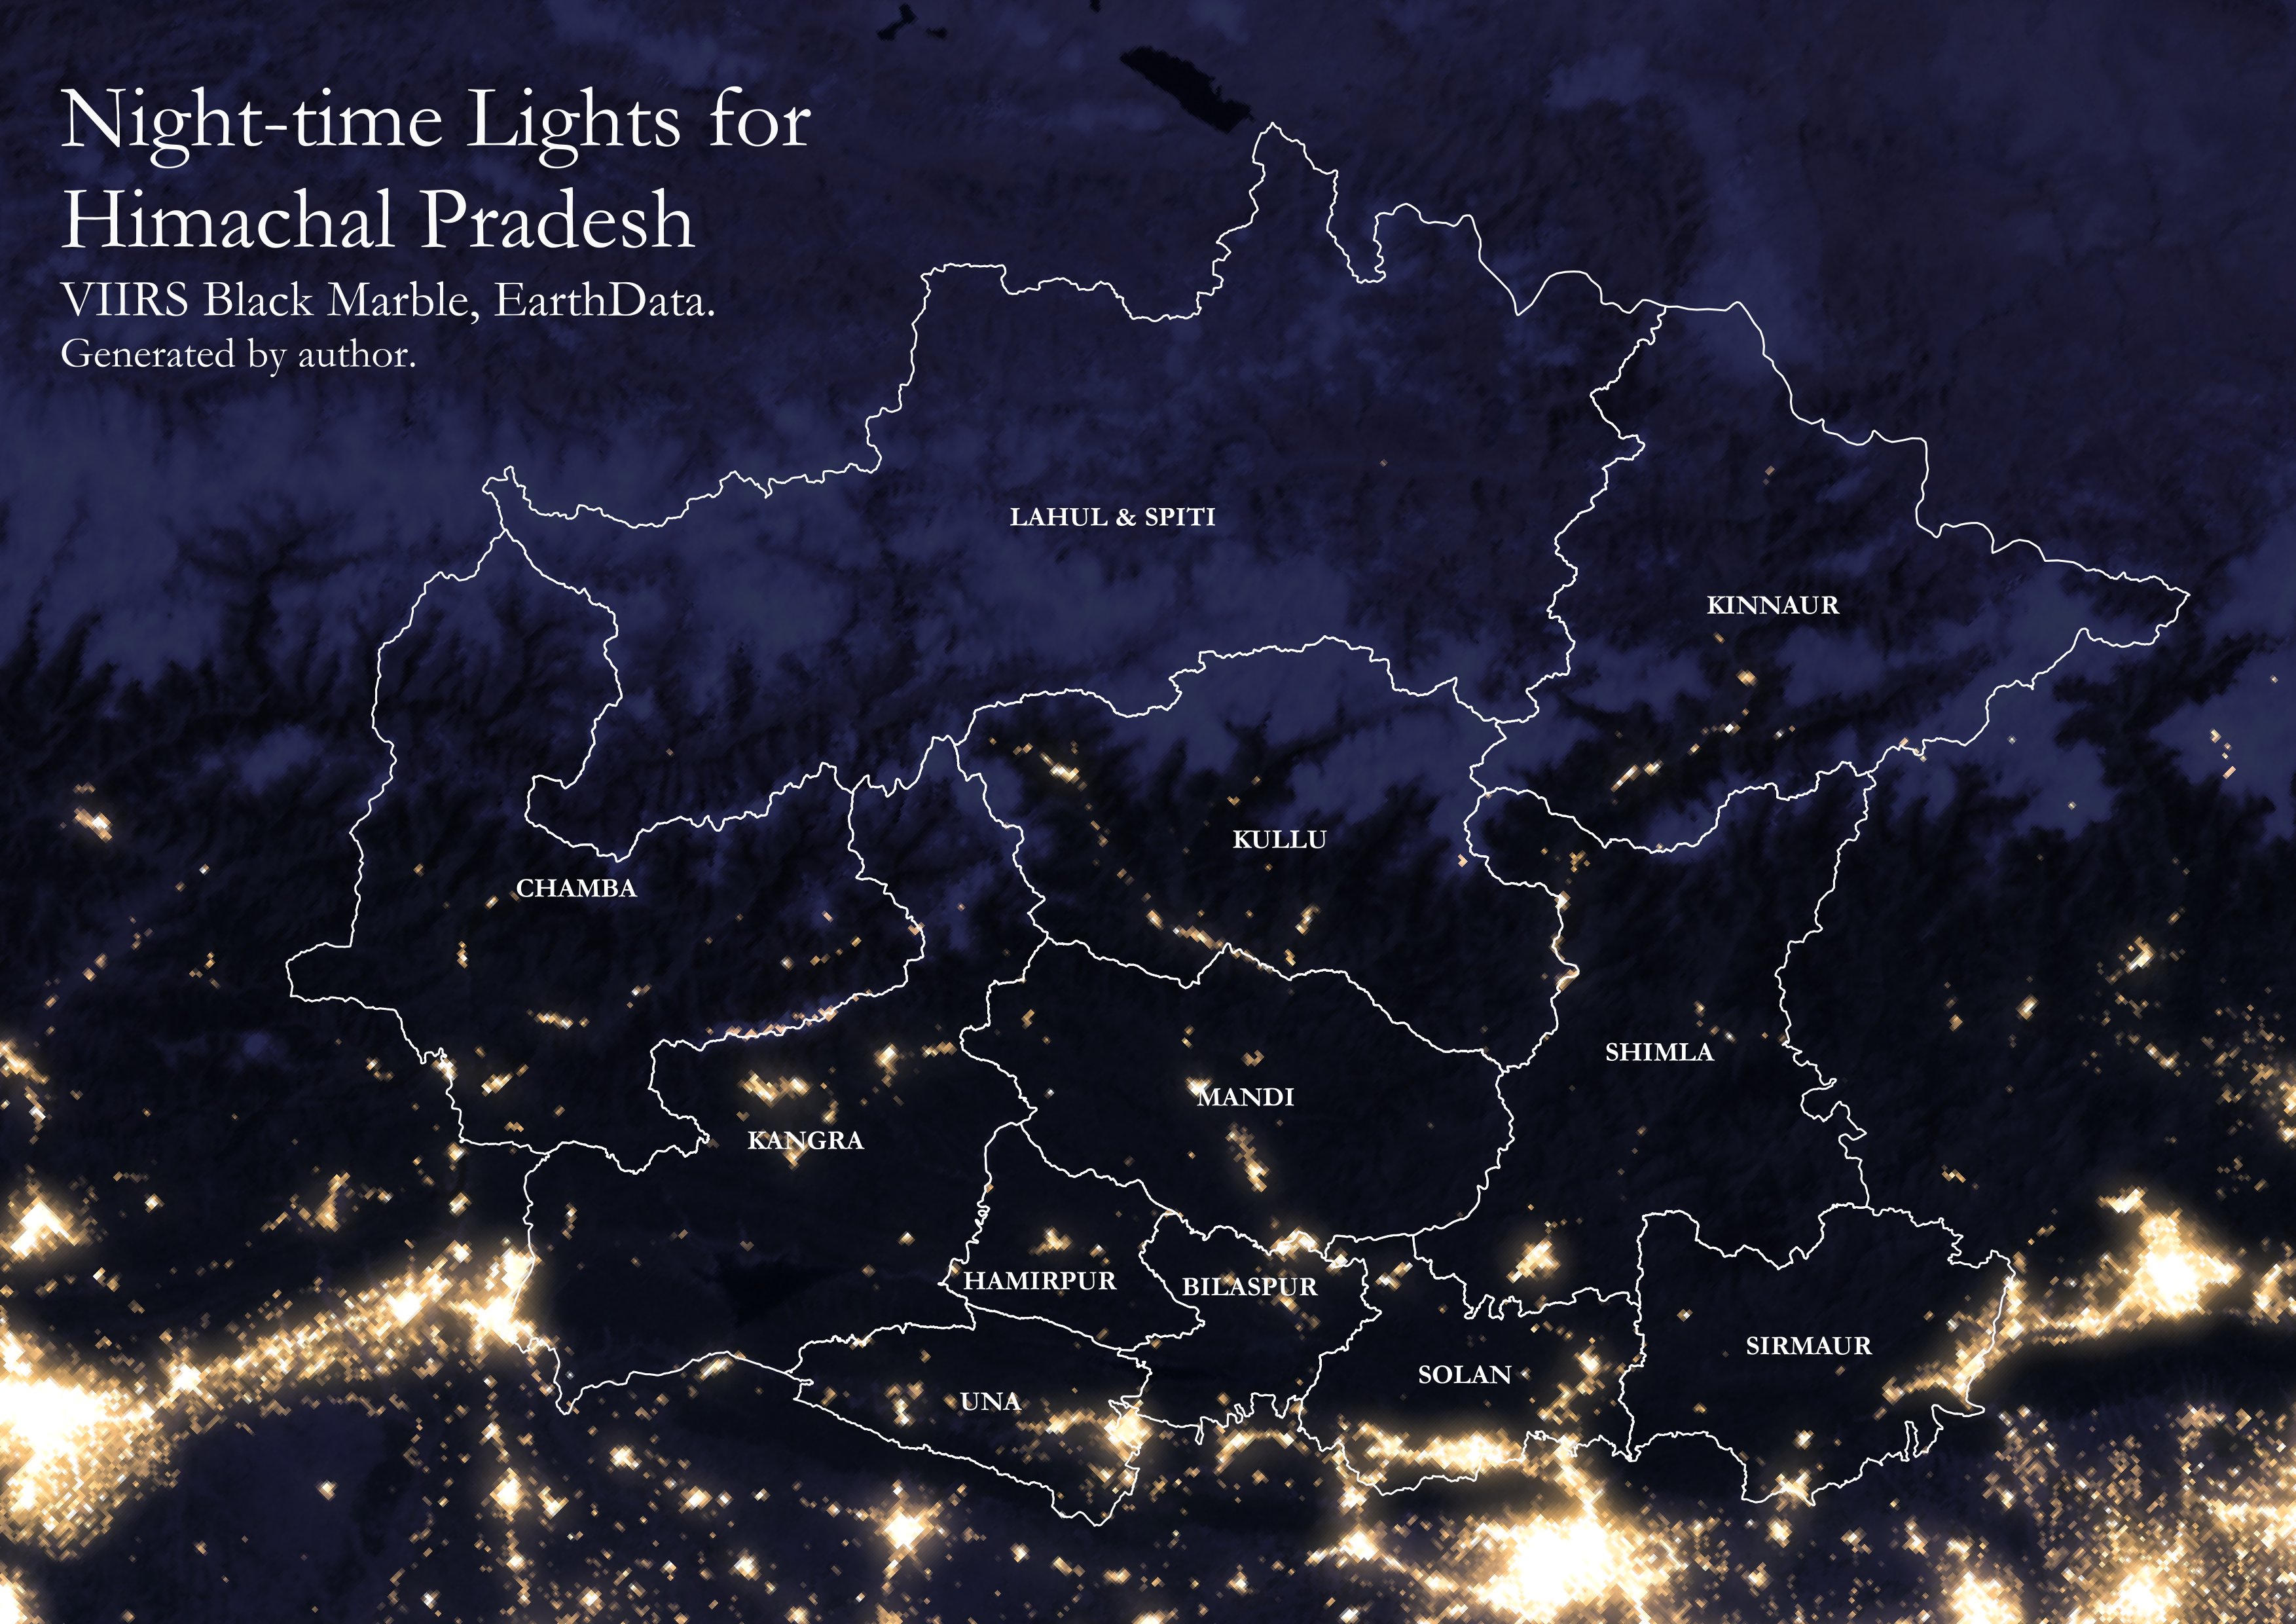
\includegraphics[width=0.85\textwidth]{images/ntl_hp.png}
    \caption{Nighttime lights for Himachal Pradesh.}
    \end{center}
\end{figure*}

\subsubsection*{Uttarakhand}

\begin{description}
    \item[Forest Cover] The state exhibits a heterogeneous pattern of forest cover growth. From the early 2000s to the mid-2000s, the trend mirrored that of Himachal Pradesh, with increasing forest cover in the northern districts and a decline in the southern districts, notably Haridwar and Rudrapur. However, from the mid-2000s to the 2010s, the forest cover decreased across the state. After 2010, a resurgence in forest cover growth was observed.
    \item[Nighttime lights] Nighttime lights increased gradually from the early 2000s to the mid-2000s. However, from the mid-2000s to the early 2010s, there was a more pronounced growth in nighttime light intensity, depicting higher economic growth.

\end{description}

\subsection{Results}

We estimate a simple model of the EKC, using our compound indices across 15,466 \textit{shrids} located within the two states. First, we construct our indices with equal weights $w_i$ across variables:

\begin{align*}
    EconIndex_i = & w_1(NTL_i) + w_2(Builtup_i) \\
    EnvIndex_i = & w_1(AQI_i) + w_2(ForestCover_i) \\
                 &+ w_3(LST_i)
\end{align*}

where $\sum_{i=1}^{n}w_i = 1$ and $w_i = w_j \forall i, j$ for each Index. We then estimate a quadratic fixed-effects model in two epochs:

\begin{align*}
EnvIndex_{it} =& \beta_0 + \beta_1(EconIndex_{it}) + \beta_2(EconIndex_{it}^2) \\ 
                & + \eta_i + \epsilon_{it} 
\end{align*}

where $\eta_i$ represents individual (\textit{shrid}-specific) fixed effects and $\epsilon_{it}$ represents the stochastic error term.


\begin{table}[h]
    \centering
    \begin{tabular}{l|rrrr}
    \hline
    \multicolumn{1}{c}{\textbf{}} & \multicolumn{1}{c}{\textbf{Coef.}} & \multicolumn{1}{c}{\textbf{Std. Err.}} & \multicolumn{1}{c}{\textbf{t}} & \textbf{P\textgreater{}t} \\ \hline
    $EconIndex$                     & 0.0242\textsuperscript{***}                             & 0.0004                                 & 61.547     & 0.000                     \\ 
    $EconIndex^2$                   & -0.0002\textsuperscript{***}                            & 0.0001                                 & -18.148    & 0.000                    
    \\ \hline        
\end{tabular}
\caption{First epoch regression results. *** represent significance at the 1\% level.\label{table:reg1}}
\end{table}


\begin{table}[h]
    \centering
    \begin{tabular}{l|rrrr}
    \hline
    \multicolumn{1}{c}{\textbf{}} & \multicolumn{1}{c}{\textbf{Coef.}} & \multicolumn{1}{c}{\textbf{Std. Err.}} & \multicolumn{1}{c}{\textbf{t}} & \textbf{P\textgreater{}t} \\ \hline
    $EconIndex$                     & -0.2366\textsuperscript{***}                             & 0.0332                                 & -7.1136     & 0.000                     \\ 
    $EconIndex^2$                   & 0.0073\textsuperscript{***}                            & 0.0016                                 & 4.7800    & 0.000                    
    \\ \hline        
\end{tabular}
\caption{Second epoch regression results. *** represent significance at the 1\% level.\label{table:reg2}}
\end{table}


The regression results showcase a mixed response with respect to the Environmental Kuznets curve hypothesis. During the initial epoch (Table~\ref{table:reg1}), the results are consistent with the EKC and scatterplot is an inverse-U shaped curve, that is economic growth and environment degradation, are both increasing until a certain level before the environment degradation starts to reduce.

With time, there is a deviation from this hypothesis. During the second epoch (Table~\ref{table:reg2}), the results contradicted the EKC, with a U-shaped curve indicating that as economic growth increases there is a fall in environmental degradation till a certain level. After that certain level is attained, the environmental degradation starts to rise again with economic growth.

\begin{figure}[h]
    \centering
    \includegraphics[width=0.4\textwidth]{images/kuznets.png}
    \caption{Estimated relationship for first epoch, similar to the EKC from Figure 1.}
\end{figure}

\begin{figure}[h]
    \centering
    \includegraphics[width=0.4\textwidth]{images/notkuznets.png}
    \caption{Estimated relationship for second epoch, inverse of Figure 3.}
\end{figure}



\section{Conclusion}

We find that there exists significant complexity and geography-specific heterogeneity in the relationship between economic development and environmental degradation. It depends upon the time period and the data being looked at. Sustainable development is thus incumbent upon understanding the needs of the economy at the time period concerning the policy decision. There is no ‘one size fits all’ policy that can work at all periods without any alteration.

The literature on development, as well as the lived experiences of several developing economies tell us that it is natural to face high environmental degradation during high economic growth (as backed up by the EKC), but after a certain time period, the focus should be shifted to growth without harming the environment. 

Macroeconomic theory tells us that if the economy is facing a U-shaped curve, the policymaker must focus on strategies to sustain growth while simultaneously reducing environment degradation. Simple measures include switching to renewable sources of energy, solar plants, windmills which might be financially costly for developing countries but as a country attains growth, they can invest for environment protection. Other measures include encouragement of public transport as well as a switch to electric vehicles.




\begin{acks}
We are indebted to the Development Data Lab (\hyperlink{https://www.devdatalab.org}{SHRUG}) for building and archiving several useful datasets on India. We thank Dr Gopal Krishna Roy for his encouragement and comments.
\end{acks}

\begin{dci}
The authors declared no potential conflicts of interest with respect to the research, authorship, and/or publication of this article.
\end{dci}

\begin{funding}
The authors received no financial support for the research, authorship, and/or publication of this article.
\end{funding}
% \begin{thebibliography}{99}
% \bibitem[Kopka and Daly(2003)]{R1}
% Kopka~H and Daly~PW (2003) \textit{A Guide to \LaTeX}, 4th~edn.
% Addison-Wesley.

% \bibitem[Lamport(1994)]{R2}
% Lamport~L (1994) \textit{\LaTeX: a Document Preparation System},
% 2nd~edn. Addison-Wesley.

% \bibitem[Mittelbach and Goossens(2004)]{R3}
% Mittelbach~F and Goossens~M (2004) \textit{The \LaTeX\ Companion},
% 2nd~edn. Addison-Wesley.

% \end{thebibliography}

\theendnotes

\end{document}
